
\documentclass[12pt,a4paper]{amsart}
% ukazi za delo s slovenscino -- izberi kodiranje, ki ti ustreza
\usepackage[slovene]{babel}
%\usepackage[cp1250]{inputenc}
\usepackage[T1]{fontenc}
\usepackage[utf8]{inputenc}
\usepackage{amsmath,amssymb,amsfonts}
\usepackage{url}
\usepackage{graphicx}
%\usepackage[demo]{graphicx}
%\usepackage[normalem]{ulem}
\usepackage[dvipsnames,usenames]{color}

% ne spreminjaj podatkov, ki vplivajo na obliko strani
\textwidth 15cm
\textheight 24cm
\oddsidemargin.5cm
\evensidemargin.5cm
\topmargin-5mm
\addtolength{\footskip}{10pt}
\pagestyle{plain}
\overfullrule=15pt % oznaci predlogo vrstico


% ukazi za matematicna okolja
\theoremstyle{definition} % tekst napisan pokoncno
\newtheorem{definicija}{Definicija}[section]
\newtheorem{primer}[definicija]{Primer}
\newtheorem{opomba}[definicija]{Opomba}

\renewcommand\endprimer{\hfill$\diamondsuit$}


\theoremstyle{plain} % tekst napisan posevno
\newtheorem{lema}[definicija]{Lema}
\newtheorem{izrek}[definicija]{Izrek}
\newtheorem{trditev}[definicija]{Trditev}
\newtheorem{posledica}[definicija]{Posledica}


% za stevilske mnozice uporabi naslednje simbole
\newcommand{\R}{\mathbb R}
\newcommand{\N}{\mathbb N}
\newcommand{\Z}{\mathbb Z}
\newcommand{\C}{\mathbb C}
\newcommand{\Q}{\mathbb Q}

% ukaz za slovarsko geslo
\newlength{\odstavek}
\setlength{\odstavek}{\parindent}
\newcommand{\geslo}[2]{\noindent\textbf{#1}\hspace*{3mm}\hangindent=\parindent\hangafter=1 #2}

% naslednje ukaze ustrezno popravi
\newcommand{\program}{Matematika} % ime studijskega programa: Matematika/Finan"cna matematika
\newcommand{\imeavtorja}{Klemen Hovnik\\ Matija Gubanec Hančič \\ Jan Rudof} % ime avtorja
\newcommand{\imementorja}{Riste} % akademski naziv in ime mentorja
\newcommand{\naslovdela}{Predpisana drevesa z najmanjšim/največjim Wienerjevim indeksom}
\newcommand{\letnica}{2018} %letnica 


% vstavi svoje definicije ...




\begin{document}

% od tod do povzetka ne spreminjaj nicesar
\thispagestyle{empty}
\noindent{\large
UNIVERZA V LJUBLJANI\\[1mm]
FAKULTETA ZA MATEMATIKO IN FIZIKO\\[5mm]
\program\ -- 1.~stopnja}
\vfill

\begin{center}{\large
\imeavtorja\\[2mm]
{\bf \naslovdela}\\[10mm]
Projekt v povezavi z OR\\[1cm]}

\end{center}
\vfill

\noindent{\large
Ljubljana, \letnica}
\pagebreak

\thispagestyle{empty}
\tableofcontents
\pagebreak

\section{Navodilo}

We want to analyze the structure of trees on a fixed number of vertices $n$ and fixed maximum
degree $\Delta$ that have Wiener index (i.e. total distance) as small as possible. Similarly, we want to
find the structure of trees on a fixed number of vertices $n$ with fixed diameter $d$ that have Wiener
index (i.e. total distance) as large as possible.
In order to get the answer for very small values of $n$ first, apply an exhaustive search, and
next, for larger $n$, apply a genetic algorithm or any other metaheuristic. Verify for how large $n$
your exhaustive search and your genetic algorithm implementations are efficient.




\section{Uvod}

Naj bo $G=(V(G),  E(G))$ enostaven povezan neusmerjen graf. $Wienerjev$ $ indeks$ (oziroma $Wienerjevo$  $"stevilo$ $ W(G)$) je definiran kot
\begin{equation}
W(G) = \frac{1}{2}\sum_{u\in V(g)}\sum_{v\in V(g)} d_G(u,v).
\end{equation}
Tukaj označimo z $d_G(u,v)$ razdaljo med vozliščem $u$ in $v$ v grafu $G$. 
\\
\\
Naša naloga je, da analiziramo lastnosti dreves z določenim številom vozlišč in 
fiksno maksimalno stopnjo vozlišč, ki imajo najmanjši Wienerjev indeks. Podobno nas zanimajo tudi lastnosti 
dreves na določenem številu vozlišč s fiksnim premerom, ki imajo največji možni Wienerjev indeks.
\\
\\
Za izvedbo projekta smo si izbrali programski jezik $Sage$, saj ta že vsebuje orodja za delo z grafi, prav tako 
pa ima tudi generator dreves in že vgrajeno funkcijo za izračun Wienerjevega indeksa. 

\section{Opis dela}

\

Najprej smo se lotili izračuna Wienerjevih indeksov na preprostih grafih z malo vozlišči, da vidimo, kako naj bi ta struktura grafov 
z minimalnimi oziroma maksimalnimi indeksi izgledala v splošnem. 
\subsection{Enostaven algoritem}
\subsubsection{Maksimalen Wiener index na drevesih s fiksnim polmerom}
\
\\
Definirali funkcijo $drevesa(n)$, ki nam izpiše seznam vseh dreves s številom vozlišč $n$. Potem smo to funkcijo uporabili v 
funkciji $drevesa\_premer(n)$, ki nam iz prejšnjih dreves generira slovar, kjer so ključi možni premeri naših dreves, vrednosti ključev pa so pripadajoča drevesa. Tako smo si pripravili podlago za enostaven algoritem iskanja maksimalnega Weiner indexa za drevesa z določenim premerom. 
Sestavili smo funkcijo $max\_Weinerindex(n,N)$, kjer je $N$ fiksen premer. Ta funkcija nam je za vsa drevesa s številom vozlišč $n$ in premerom $N$ izpisala maksimalni Wiener index in nam to drevo tudi izrisala.
\begin{figure*}[ht]
\centering
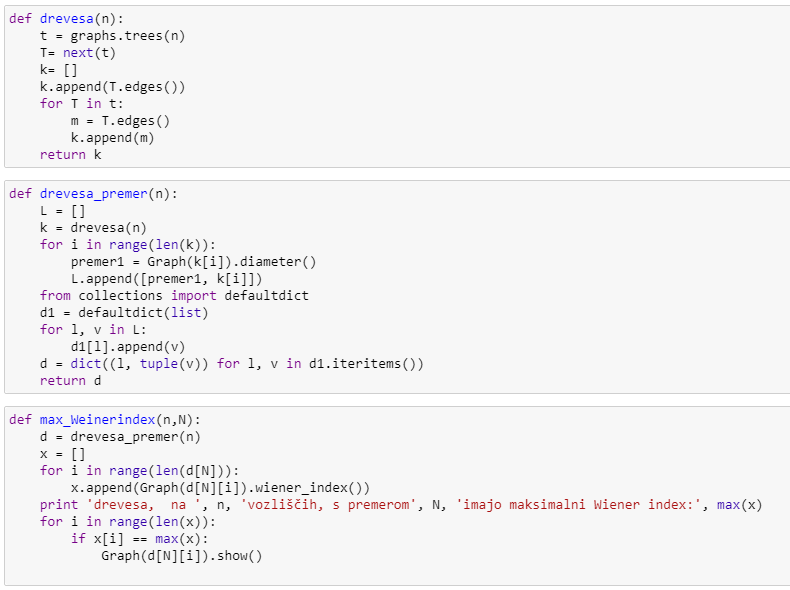
\includegraphics[width=1\textwidth]{slika1}
%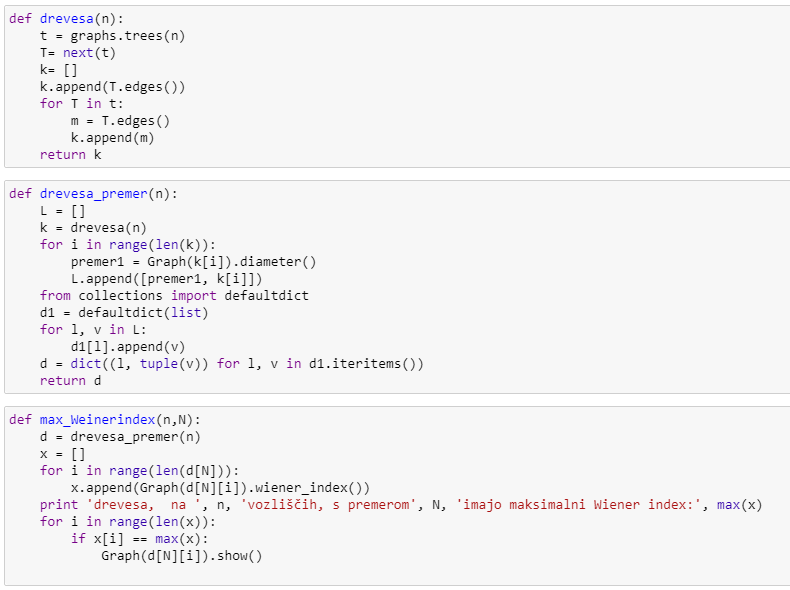
\includegraphics{slika1}
\end{figure*}
\pagebreak


\subsubsection{Minimalen Wiener index na drevesih s fiksno stonjo}
\
\\
Za iskanje najmanjših Wienerjevih indeksov pri določenem številu vozlišč $n$ in pri fiksni maksimalni stopnji  $m$
smo definirali funkcijo $fiksna\_stopnja$,  ki nam je iz seznama, ki ga vrne funkcija $drevesa(n)$ izpisala drevesa z maksimalno stopnjo $m$. Izmed teh optimalnih dreves pa smo potem s funkcijo $.wiener\_index()$ izračunali najmanjši Wiener index, ter drevo s tem indeksom tudi izpisali.

\begin{figure*}[ht]
\centering
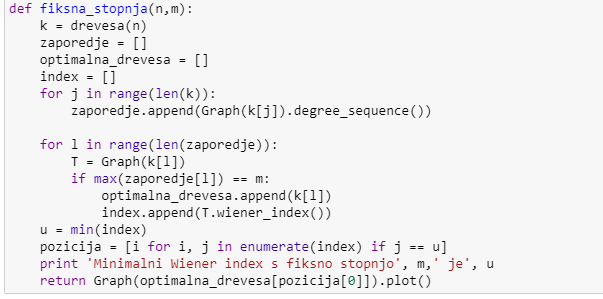
\includegraphics[width=1\textwidth]{slika2}
\end{figure*}
\pagebreak
\
\\
Hitro smo prišli do ugotovitve, da je naš algoritem za izračun indeksov časovno prepotraten. Zato smo se problema iskanja Wienerjevih indeksov lotili na drugačen način. In sicer z $genetskim algoritmom$ katerega ideja je, da izmed dreves na manjših vozliščih gradimo večja drevesa


\subsection{Genetski algoritem}
\
\\
$Genetski$ $algoritem$ je metahevristika, navdihnjena s strani procesov naravne selekcije in spada v razred $razvojnih$
$algoritmov$. Uporablja se za generiranje kvalitetnih rešitev v optimizaciji, ki temeljijo na operatorjih kot so mutacija, križanje
in selekcija.  
\\
\\
V genetskem algoritmu se uporabi množica kandidatov za rešitev, ki jih nato razvijamo do optimalne rešitve. Vsak kandidat
ima določene lastnosti, katere lahko spremenimo oziroma lahko mutirajo. Evolucija rešitev se ponavadi začne na naključni izbiri kandidatov,
katere potem s pomočjo iteracije razvijamo. Na vsakem iterativnem koraku se potem oceni primernost novih kandidatov za optimizacijski
problem. Najboljše kandidate potem uporabimo za naslednji korak iteracije in tako dalje. Na koncu se algoritem zaključi,
ko doseže maksimalno število iteracijskih korakov oziroma, ko dobi najboljši približek optimalni rešitvi.
\\
\\
Naša začetna množica kandidatov bodo optimalna drevesa, ki smo jih dobili z našim prvim enostavnim algoritmom. 
Nato bomo ustvarili genetski algoritem, ki bo iz teh začetnih podatkov generiral nova optimalna drevesa. Ta postopek bomo
nadaljevali (in pri tem selekcionirali iz novo nastalih dreves le najboljše za naslednje korake), dokler ne bomo prišli do optimalnih 
dreves za določeno število vozlišč. Pri tem bomo morali paziti, da se bo ohranjala maksimalna stopnja vozlišč, 
oziroma v drugem primeru, premer. 
\\
\\
Na koncu bomo primerjali algoritma in pogledali, kdaj se ustavi naš enostavni algoritem za iskanje grafov z max/min Wienerjevim indeksom
oziroma za katero število vozlišč je genetski algoritem še učinkovit.





\end{document}